\documentclass[11pt, a4paper, oneside]{memoir}                                                      %%

\usepackage[utf8]{inputenc}
\usepackage[ngerman]{babel}     % new german spelling, umlauts and other regional settings like date format
\usepackage[shortlabels]{enumitem}
\usepackage{nameref,zref-xr}
\zxrsetup{toltxlabel}
\usepackage{graphicx}           % allow for inclusion of images
\usepackage[table,svgnames]{xcolor} % define colors
\usepackage{url}                % weblinks, etc.
\usepackage{colortbl}           % colored table cells
\usepackage{longtable}          % tables, which are longer than one page
\usepackage{hyperref}
\usepackage[intlimits]{mathtools}
\hypersetup{
	bookmarksopen=true,                       % expand bookmark tree in acrobat by default
	pdftitle={SEPMP},                         % set title in meta pdf information
	pdfauthor={Teilnehmer 1, Teilnehmer 2, Teilnehmer 3},                             % set author in meta pdf information
	pdfsubject={},                            % set subject in meta pdf information
	pdfkeywords={},                           % set keyword list in meta pdf information
	colorlinks=true,                          % use colored links instead of black ones
	linkcolor=blue,                           % color for internal links
	anchorcolor=black,                        % color for anchor links
	citecolor=black,                          % color for bibliography links
	filecolor=magenta,                        % color for system local links
	urlcolor=blue,                            % color for url links
	plainpages=false,                         % must be false, so that PDF bookmarks work properly
	hypertexnames=false,                      % use guessable names for links; used for correct bookmarks
	linktocpage                               % link page numbers in toc instead of section names
}
\makeatletter
\def\namedlabel#1#2{\begingroup
    #2%
    \def\@currentlabel{#2}%
    \phantomsection\label{#1}\endgroup
}
\makeatother

\newenvironment{lhp}[3]%
{%
	\item [\namedlabel{#3}{/#2\arabic{#1}/}]% \hfill%
	\addtocounter{#1}{10}%
	\begin{description}[leftmargin=0cm, style=sameline]%
}%
{%
	\end{description}%
}

\newenvironment{php}[4]%
{%
	\item [\namedlabel{#4}{/#2\arabic{#1}/} (\ref{#3})] \hfill%
	\addtocounter{#1}{10}%
	\begin{description}[style=sameline]%
}%
{%
	\end{description}%
}

\zexternaldocument*{Lastenheft}

\makeatletter
	\newcommand{\mysubject}{Pflichtenheft}
	\newcommand{\mygroup}{Gruppe N}
	\newcommand{\myauthor}{%
		Teilnehmer 1 \\
		Teilnehmer 2 \\
		Teilnehmer 3 \\
		Teilnehmer 4 \\
		Teilnehmer 5 %
	}
\makeatother

\begin{document}

	\thispagestyle{empty}
	\newcommand{\Rule}{\rule{\textwidth}{0.5mm}}
	\begin{center}
	% upper part
	{\Large 
\includegraphics[height=20mm]{img/TUKL_LOGO_4C} \par}

	\vspace{0.5em}

	{\Large AG Computergrafik \& HCI \\ apl. Prof. Dr. Achim Ebert \par}

	\vspace{0.5em}

	{\Large SEP/MP \the\year \par}


	\vspace{5cm}

	% middle part
	\Rule

	\vspace{1cm}

	{\Huge Exploding Kittens \par}

	\vspace{0.5em}

	{\Large \mysubject \par}

	\vspace{0.5em}

	{\small \today \par}

	\vspace{0.7cm}

	\Rule


	\vfill %%%%%%%%%%%%%%%%%%%%%%%%%%%%%%%%%%%%%%%%%%%%%%%%%%%%%%%%%%%%%%%%


	% lower part
	\emph{\textbf{\mygroup}} \\[1em]
	\myauthor

	\end{center}


	\tableofcontents

	\chapter{Projekttreiber}

\section{Projektziel}

Im Rahmen des Software-Entwicklungs-Projekts/Modellierungspraktikums {\the\year} soll ein einfach zu bedienendes Client-Server-System zum Spielen von Exploding Kittens über ein Netzwerk implementiert werden. Die Benutzeroberfläche soll intuitiv bedienbar sein.

\section{Stakeholders}

\newcounter{sh}\setcounter{sh}{10}

\begin{description}[leftmargin=5em, style=sameline]
	
	\begin{lhp}{sh}{SH}{sh:Spieler}
		\item [Name:] Spieler
		\item [Beschreibung:] Menschliche Spieler.
		\item [Ziele/Aufgaben:] Das Spiel zu spielen.
	\end{lhp}
	
	\begin{lhp}{sh}{SH}{bsh:Spieler}
		\item [Name:] Eltern
		\item [Beschreibung:] Eltern minderjähriger Spieler.
		\item [Ziele/Aufgaben:] Wollen Spielzeit ihrer Kinder begrenzen und Zugriff auf sensible Inhalte kontrollieren.
	\end{lhp}
	
	\begin{lhp}{sh}{SH}{bsh:gesetzgeber}
		\item [Name:] Gesetzgeber
		\item [Beschreibung:] Das Amt für Jugend und Familie.
		\item [Ziele/Aufgaben:] Die Rechte der Spieler schützen und gewähren indem er Gesetze erstellt. 
	\end{lhp}
	
	\begin{lhp}{sh}{SH}{bsh:investor}
		\item [Name:] Investoren (nur für Beispielzwecken)
		\item [Beschreibung:] Parteien, die das Finanzmittel für die Entwicklung des Systems bereitstellen.
		\item [Ziele/Aufgaben:] Gewinn zu erzielen, indem das System an Endverbraucher verkauft wird.
	\end{lhp}
	
	\begin{lhp}{sh}{SH}{bsh:betreuer}
		\item [Name:] Betreuer
		\item [Beschreibung:] HiWis, die SEP/MP Projektgruppen betreuen.
		\item [Ziele/Aufgaben:] Die Spielentwicklung durch die Studenten betreuen
	\end{lhp}
	
	\begin{lhp}{sh}{SH}{bsh:prof}
		\item [Name:] Prof. Dr. Achim Ebert
		\item [Beschreibung:] Leiter des Software-Entwicklunsprojekt
		\item [Ziele/Aufgaben:]  Leitung der Lehrverantstaltung
	\end{lhp}
		
\end{description}

\section{Aktuelle Lage}

Aktuell gibt es nur eine physische Form des Spiels und eine App für mobile Endgeräte. Da es zur Zeit keine Version des Spiels für Desktop-Computer gibt entsteht die Problematik, dass ein potenzieller Spieler ohne ein entsprechendes Handy keine Möglichkeit besitzt am Spiel teilzunehmen. Die physischen Spielkarten weisen außerdem das Problem auf, dass sie sich bei häufigem Gebrauch abnutzen oder kaputt gehen. \\Dieses Projekt soll solchen Spielern ermöglichen ohne Handy online miteinander zu spielen und einer überhöhten Kartenabnutzung vorzubeugen. Es leistet somit auch einen Beitrag zur Müllvermeidung. \\Eltern können das Spielverhalten ihrer Kinder in dieser Version genauer kontrollieren als bei den oben Genannten Varianten. \\Investoren profitieren durch die Spielverkäufe an so neu gewonnene Spieler. 
	\chapter{Projektbeschränkungen}

\section{Beschränkungen}

\newcounter{lb}\setcounter{lb}{10}

\begin{description}[leftmargin=5em, style=sameline]
	
	\begin{lhp}{lb}{LB}{beschr:lehrbots}
		\item [Name:] Selbstlehrende Bots
		\item [Beschreibung:] Keine Selbstlehrfunktion von Bots wird implementiert.
		\item [Motivation:] Die Funktionalität ist zu aufwändig zu implementieren und passt deshalb nicht in das Zeitbudget.
		\item [Erfüllungskriterium:] Intelligenzalgorithmus von Bots ist so vorprogrammiert, dass sie Entscheidungen nur anhand des vorprogrammierten Wissens sowie des aktuellen Spielstands treffen, ohne dabei frühere Spiele zu berücksichtigen.
	\end{lhp}
	
	\begin{lhp}{lb}{LB}{beschr:anwendungsbereich}
		\item [Name:] Anwendungsbereich
		\item [Beschreibung:] Das System ist ausschließlich für den privaten Bereich ausgelegt.
		\item [Motivation:] Firmen oder kommerzielle Anwender haben wenig Verwendung für ein digitales Kartenspiel. 
		\item [Erfüllungskriterium:] Auslegung auf privaten Bereich
	\end{lhp}
	
		
	\begin{lhp}{lb}{LB}{beschr:implsprache}
		\item [Name:] Implementierungssprache
		\item [Beschreibung:] Für die Implementierung ist ausschließlich Java 8 oder höher zu verwenden.
		\item [Motivation:] Das optimiert die Betreuung von SEP/MP und koordiniert die Mitarbeit.
		\item [Erfüllungskriterium:] Quellcode in Java
	\end{lhp}
	
	\begin{lhp}{lb}{LB}{beschr:gui}
		\item [Name:] GUI-Framework
		\item [Beschreibung:] Die GUI ist mit JavaFX zu realisieren.
		\item [Motivation:] Das optimiert die Betreuung von SEP/MP und koordiniert die Mitarbeit.
		\item [Erfüllungskriterium:] Verwendung von JavaFX
	\end{lhp}
	
	\begin{lhp}{lb}{LB}{beschr:gitlab}
		\item [Name:] Gitlab
		\item [Beschreibung:] Für die Entwicklung ist das vorgegebene GitLab-Repository zu verwenden.
		\item [Motivation:] Das optimiert die Betreuung von SEP/MP und koordiniert die Mitarbeit.
		\item [Erfüllungskriterium:] Benutzen des GitLab-Repository
	\end{lhp}
	
	
\end{description}

\section{Glossar}

\begin{center}
	\rowcolors{2}{Gray!15}{White}
	\begin{longtable}{p{0.25\textwidth} p{0.25\textwidth} p{0.4\textwidth}}
		\textbf{Deutsch} & \textbf{Englisch} & \textbf{Bedeutung} \\
		\hline \hline \endhead
		Beispiele & Examples & Beispiele aus dem SEP letzter Jahren, welche angepasst werden müssen.\\
		Explosion & explosion & Teilnehmer, die explodieren verlieren. \\    
		Karte & card & Spielkarte, die in einem Zug gespielt werden kann\\
		Entschärfung & defuse & Mit dieser Karte kann sich ein Spieler vor einer Explosion retten\\
		Exploding Kitten & Exploding Kitten & Wer diese Karte zieht explodiert\\
		Nö! & nope! & Andere Karte außer Kraft setzen\\
		Angriff & attack & Zug beenden ohne eine Karte zu ziehen, nächster Spieler muss zwei Karten ziehen\\
		Hops! & skip & Zug beenden ohne Karte zu ziehen\\
		Wunsch & favor & Mitspieler zwingen eine Karte rauszugeben\\
		Mischen & shuffle & Spielstapel neu mischen\\
		Blick in die Zukunft & See to the future & Oberste drei Karten des Spielstapels geheim ansehen\\
		Katzen-Karten & cat Cards & Als Pärchen gespielt eine zufällige Karte vom Mitspieler stehlen, als Drilling Wunschkarte stehlen, als Fünfling beliebige Karte vom Ablagestapel nehmen\\
		
		Passen & skip & Keine Karten ausspielen\\
		Spielzug & move & Eine oder mehrere Karten offen auf den Stapel legen und Anweisungen befolgen. \\
		
		Bot & bot & Spieler, dessen Spielaktionen vom Computer entschieden und durchgeführt werden\\
		Kekse & Cookies & Offiziell keine gültige Maßnahme zur Bestechung der HiWis\\          
		Lobby & lobby & Virtueller Raum zum Betreten eines Spielraums\\	
		Spiel (Regelwerk) & game & Exploding Kittens \\
		Spieler & player & Teilnehmer am Spielgeschehen\\
		Spielraum & game room & Virtueller Raum, in dem ein Spiel stattfindet\\
		Zug & turn & Zustand in dem ein Spieler eine Spielaktion ausführen muss\\
	\end{longtable}
\end{center}

\section{Relevante Fakten und Annahmen}

Wichtige gekannte Fakten und getroffene Annahmen, die sich auf das Projekt direkt oder indirekt beziehen und dadruch auf die zukünftige Implementierungsentscheidungen Effekt haben können.

\newcounter{fa}\setcounter{fa}{10}

\begin{description}[leftmargin=5em, style=sameline]
	
	\begin{lhp}{fa}{FA}{fa:fortentwicklung}
		\item [Name:] Keine Fortentwicklung des App nach SEP/MP.
		\item [Beschreibung:] Nach Ende des SEP/MP wird das Projekt nicht weiterentwickelt.
		\item [Motivation:] Das Entwicklungsteam hat keine Lust darauf.
	\end{lhp}
	
	\begin{lhp}{fa}{FA}{fa:recht}
		\item [Name:] Keine Lizenzen für Spielartefakte.
		\item [Beschreibung:] Weder die TU Kaiserslautern noch das Spielwerk + die Freizeit GmbH gewahren dem Entwicklungsteam die Rechte für die Spielartefakte.
		\item [Motivation:] Rechtliche Vorsorge.
	\end{lhp}
	
	\begin{lhp}{fa}{FA}{fa:recht-vergangenheit}
		\item [Name:] Keine bekannte Nachteile von Verwendung von Spielartefakten.
		\item [Beschreibung:] Es ist nicht bekannt, dass die SEP/MP-Teilnehmer der letzten Jahre irgendwelche rechtlichen Probleme dadurch gehabt haben, dass sie die Spielartefakten vom Spielwerk + Freizeit GmbH im Rahmen ihrer SEP/MP eingesetzt haben.
		\item [Motivation:] Rechtliche Vorsorge.
	\end{lhp}
	
	
\end{description}


	\chapter{Funktionale Anforderungen}

%\section{Systemkontext}

\section{Systemfunktionen}

\newcounter{pfc}\setcounter{pfc}{10}

\begin{description}[leftmargin=5em, style=sameline]
	
	\begin{lhp}{pfc}{LF}{funk:spielverw}
		\item [Name:] Spielverwaltung
		\item [Beschreibung:] Das System verwaltet von mehreren Spielern geteilte Spiele in einem Spielraum. Spiele erfolgen nach den Spielregeln.
	\end{lhp}
	
	\begin{lhp}{pfc}{LF}{funk:zugriff}
		\item [Name:] Zugriffsverwaltung
		\item [Beschreibung:] Das System verwaltet den Zugang zum Spiel anhand von Benutzerdaten. Spieler können sich registrieren, anmelden, abmelden sowie ihre Kontos löschen.
	\end{lhp}

	\begin{lhp}{pfc}{LF}{funk:spielraum}
		\item [Name:] Verwaltung der Spielräume
		\item [Beschreibung:] Das System verwaltet die Erstellung, Änderung und Löschung der Spielräume.
	\end{lhp}
	
	\begin{lhp}{pfc}{LF}{funk:bestenliste}
		\item [Name:] Bestenliste
		\item [Beschreibung:] Die Anzahl der gewonnen Spiele aller Spieler anzeigen.
	\end{lhp}
	
	\begin{lhp}{pfc}{LF}{funk:bots}
		\item [Name:] Intelligente Bots
		\item [Beschreibung:] Vom System gesteuerte Spieler, die möglichst gewinnbringende Strategien verfolgen. Eine leichtere und eine komplexere Version stehen zur Auswahl und können bei der Erstellung des Spielraums hinzugefügt werden.
	\end{lhp}
	
	\begin{lhp}{pfc}{LF}{funk:chat}
		\item [Name:] Chat
		\item [Beschreibung:] Möglichkeit für Spieler in der Lobby miteinander zu kommunizieren und Spielpartner zu finden. Zusätzlicher Chat für Spielräume.
	\end{lhp}

\end{description}



	\begin{figure}
\centering	
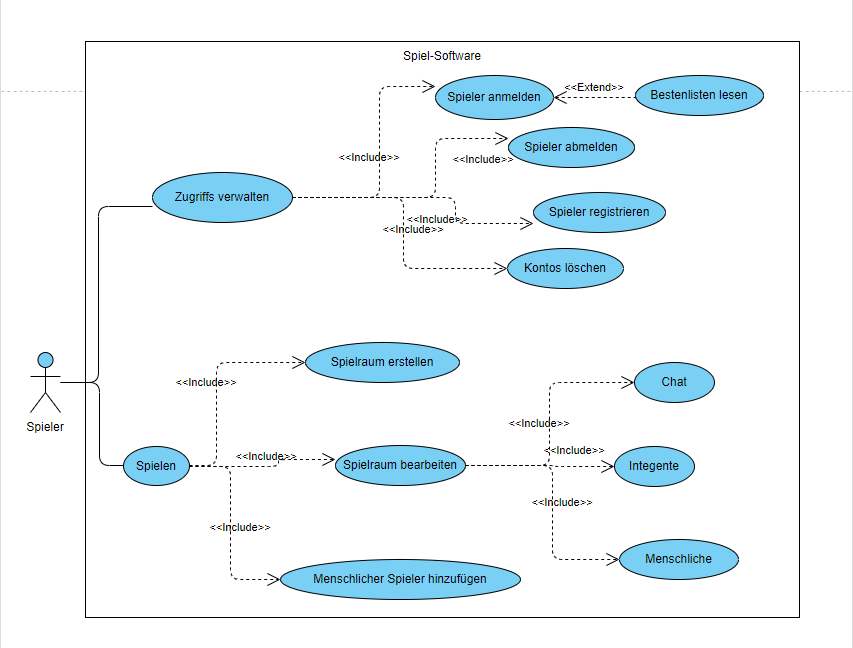
\includegraphics[width=0.9\textwidth]{img/group6.png}
\label{fig:sys}
\caption{Use Case Diagramm}
\end{figure}

\section{Systemgrenze (Use Case Diagramm)}

Die Systemgrenze wird in der Abbildung~\ref{fig:sys} dargestellt. 


\section{Beschreibungen der Anwendungsfälle}


\newcounter{uc}\setcounter{uc}{10}

\begin{description}[leftmargin=5em, style=sameline]

	\begin{lhp}{uc}{UC}{uc:zugriff}
		\item [Name:] Zugriff verwalten.
		\item [Ziel:] Zugriffsverwaltung.
		\item [Akteure:] Das System.
		\item [Vorbedingungen:] Falls vorhanden, Benutzername und Passwort. Falls nicht vorhanden, keine.
		\item [Eingabedaten:] Falls vorhanden, Benutzername \ref{daten:benutzername} und Passwort \ref{daten:passwort}. Falls nicht vorhanden, keine.
		\item [Beschreibung:] \hfill\\ Falls schon registriert:\hfill\\
		1. Der Spieler gibt der Benutzername und das Passwort.\\
		2. System prüft die Richtigkeit der Daten.\\
		\hfill\\ Falls nicht registriert:\hfill\\
		siehe \ref{uc:registrieren}
		\item [Ausnahmen:] \hfill
		\begin{itemize} 
		\item[] \textit{Benutzername und Passwort passen nicht zusammen:} Das System gibt dem Spieler einen Hinweis.				\item[] \textit{Noch nicht registriert:} siehe \ref{uc:registrieren}.
		
	\end{itemize}
	
		\item [Ergebnisse und Outputdaten:] Das Spieler hat sich erfolgreich angemeldet.
		\item [Systemfunktionen] \ref{funk:zugriff}.
	\end{lhp}

	\begin{lhp}{uc}{UC}{uc:registrieren}
	    \item [Name:] Spieler registieren.
	    \item [Ziel:] Spieler registiert sich.
	    \item [Akteure:] Spieler.
	    \item [Vorbedingungen] Keine.
        \item [Eingabedaten:] Name\ref{daten:benutzername}, Passwort\ref{daten:passwort}, Email\ref{daten:email}. 
	\item [Beschreibung:] \hfill\\ \hfill\\
	1. Spieler sendet das Formular ab.\\
	2. Das System prüft ob der Benutzername schon vorhanden ist\\	
	3. Spieler erfolgreich registiert.\\			
	\item [Ausnahmen:]\hfill 
	\begin{itemize} 
		\item[] \textit{Benutzername schon vorhanden:} Das System zeigt eine Fehlermeldung an und Spieler sendet das Formular mit anderem Benutzername ab.					
		
	\end{itemize}
	\item [Ergebnisse und Outputdaten:] Spieler erfolgreich registiert.	
	\item [Systemfunktionen:] \ref{funk:zugriff}.
    \end{lhp}
	
	\begin{lhp}{uc}{UC}{uc:anmeld}
		\item [Name:] Spieler anmelden.
		\item [Ziel:] Spieler meldet sich im System an.
		\item [Akteure:] Spieler.
		\item [Vorbedingungen] Spieler ist erfolgreich angemeldet.
		\item [Eingabedaten:] Zugriffsdaten~\ref{daten:benutzername}~\ref{daten:passwort}.
		\item [Beschreibung:] \hfill\\ \hfill\\
			1. Spieler sendet das Formular ab.\\
			2. Das System prüft die Gültigkeit von Zugangsdaten.\\				
		\item [Ausnahmen:]\hfill 
	    	\begin{itemize} 
			    \item[] \textit{Passwort oder Benutzername ist falsch:} Das System zeigt eine Fehlermeldung an.					
			
		    \end{itemize}
		\item [Ergebnisse und Outputdaten:] Spieler erfolgreich angemeldet.	
		\item [Systemfunktionen:] \ref{funk:zugriff}.
	\end{lhp}
	
	\begin{lhp}{uc}{UC}{uc:namechange}
		\item [Name:] Benutzername ändern.
		\item [Ziel:] Spieler ändert seinen Benutzername.
		\item [Akteure:] Spieler.
		\item [Vorbedingungen] Spieler ist erfolgreich angemeldet.
		\item [Eingabedaten:] Zugriffsdaten~\ref{daten:benutzername}~\ref{daten:passwort}.
		\item [Beschreibung:] \hfill\\ \hfill\\
			1. Spieler sendet das Formular ab.\\
			2. Das System prüft die Gültigkeit von Zugangsdaten.\\				
		\item [Ausnahmen:]\hfill 
	    	\begin{itemize} 
			    \item[] \textit{Passwort ist falsch:} Das System zeigt eine Fehlermeldung an.					
			
		    \end{itemize}
		\item [Ergebnisse und Outputdaten:] Benutzername erfolgreich geändert.	
		\item [Systemfunktionen:] \ref{funk:accountverw}.
	\end{lhp}	
	
	\begin{lhp}{uc}{UC}{uc:pwchange}
		\item [Name:] Passwort ändern.
		\item [Ziel:] Spieler ändert sein Passwort.
		\item [Akteure:] Spieler.
		\item [Vorbedingungen] Spieler ist erfolgreich angemeldet.
		\item [Eingabedaten:] Passwort~\ref{daten:passwort}.
		\item [Beschreibung:] \hfill\\ \hfill\\
			1. Spieler sendet das Formular ab.\\
			2. Das System prüft die Gültigkeit des Passworts.\\				
		\item [Ausnahmen:]\hfill 
	    	\begin{itemize} 
			    \item[] \textit{Passwort ist falsch:} Das System zeigt eine Fehlermeldung an.					
			
		    \end{itemize}
		\item [Ergebnisse und Outputdaten:] Passwort erfolgreich geändert.	
		\item [Systemfunktionen:] \ref{funk:accountverw}.
	\end{lhp}	
	
	\begin{lhp}{uc}{UC}{uc:loeschen}
		\item [Name:] Spieler löschen.
		\item [Ziel:] Spieler entfernt seine Daten aus dem System.
		\item [Akteure:] Spieler.
		\item [Vorbedingungen] Spieler erfolgreich angemeldet.
		\item [Eingabedaten:] Passwort~\ref{daten:passwort}.
		\item [Beschreibung:] \hfill\\ \hfill\\
				1. Spieler sendet das Formular ab.\\
				2. Das System prüft die Richtigkeit des Passworts und fragt Spieler noch ein mal, ob er sich wirklich aus dem System entfernen möchte.\\
				3. Spieler bestätigt seine Intention.\\
				4. Das System entfernt alle Daten des Spielers aus der Datenbank und bewegt Spieler in den Vorraum.\\
		\item [Ausnahmen:] \hfill
			\begin{itemize} 
				\item[] \textit{Keine Löschung erwünscht:} Schritt 4 wird nicht durchgeführt.
				
			\end{itemize}
		\item [Ergebnisse und Outputdaten:] Spielerkonto wurde gelöscht.	
		\item [Systemfunktionen:] \ref{funk:zugriff}.
	\end{lhp}
   
	\begin{lhp}{uc}{UC}{uc:bestenlistesehen}
    	\item [Name:] Bestenliste lesen.
    	\item [Ziel:] Spieler liest die Bestenliste.
    	\item [Akteure:] Spieler.
    	\item [Vorbedingungen] Spieler erfolgreich angemeldet.
    	\item [Eingabedaten:] keine.
    	\item [Beschreibung:] Spieler liest die Bestenliste \ref{daten:bestenliste}.
    	\item [Ausnahmen:] keine.
    	\item [Ergebnisse und Outputdaten:] Die Bestenliste wird angezeigt.	
    	\item [Systemfunktionen:] \ref{funk:bestenliste}.
    \end{lhp}

	\begin{lhp}{uc}{UC}{uc:spielen}
     	\item [Name:] Spielraum betreten.
    	\item [Ziel:] Spieler betritt Spielraum.
	    \item [Akteure:] Spieler.
    	\item [Vorbedingungen] Spieler erfolgreich angemeldet.
    	\item [Eingabedaten:] keine.
    	\item [Beschreibung:] \hfill\\ \hfill\\
    	1. Spieler wählt einen Spielraum aus und will diesem beitreten.\\
    	2. System prüft ob Spieler dem Raum beitreten kann.\\
    	3. Spieler tritt dem Raum bei oder bekommt eine Fehlermeldung.\\
    	\item [Ausnahmen:] \hfill
    	\begin{itemize} 
				\item[] \textit{Raum ist voll:} Spieler erhält eine Fehlermeldung.
				
			\end{itemize}
    	\item [Ergebnisse und Outputdaten:] Spieler in einen Spielraum.
     	\item [Systemfunktionen:] \ref{funk:spielraum}.
    \end{lhp} 

    \begin{lhp}{uc}{UC}{uc:chat}
    	\item [Name:] Chatten.
    	\item [Ziel:] Spieler chat mit einander.
    	\item [Akteure:] Spieler.
    	\item [Vorbedingungen] Spieler erfolgreich angemeldet und steht in einem Spielraum. 
    	\item [Eingabedaten:] Chatnachricht.
    	\item [Beschreibung:] \hfill\\ \hfill\\
    	1. Spieler sendet eine Nachricht.\\
    	2. System sendet Nachricht an andere Spieler.\\
    	\item [Ausnahmen:] \hfill
    	\begin{itemize} 
				\item[] \textit{Nachricht ist leer:} Schritt 2 wird übersprungen.
				
			\end{itemize}
    	\item [Ergebnisse und Outputdaten:] Chatnachricht.
    	\item [Systemfunktionen:] \ref{funk:chat}.
    \end{lhp}


    \begin{lhp}{uc}{UC}{uc:intelligentbots}
    	\item [Name:] Intelligente Bots hinzufügen.
    	\item [Ziel:] Spieler fügt ein Bot Spieler zum Spielraum.
    	\item [Akteure:] Spieler.
    	\item [Vorbedingungen] Spieler ist in einem Spielraum. 
      	\item [Eingabedaten:] keine.
    	\item [Beschreibung:] \hfill\\ \hfill\\
    	1. Spieler will einen Bot Spieler zum Spiel hinzufügen.\\
    	2. System fragt nach der Stärke des Bots.\\
    	3. Spieler gibt Präferenzen an.\\
    	4. System fügt Bot hinzu.\\
    	\item [Ausnahmen:] \hfill
    	\begin{itemize} 
				\item[] \textit{Raum ist voll:} Spieler erhält eine Fehlermeldung.
				
			\end{itemize} 
    	\item [Ergebnisse und Outputdaten:] Bot erfolgreich hinzugefügt.
    	\item [Systemfunktionen:] \ref{funk:bots}.
    \end{lhp}
    
        \begin{lhp}{uc}{UC}{uc:spielstart}
    	\item [Name:] Spielstart
    	\item [Ziel:] Alle Spieler bekommen ihre Handkarten zugeteilt und das Spiel beginnt.
    	\item [Akteure:] Spieler.
    	\item [Vorbedingungen] Spieler ist in einem Spiel. 
      	\item [Eingabedaten:] Gewünschte Karte(n).
    	\item [Beschreibung:] \hfill\\ \hfill\\
    	1. Spieler startet das Spiel aus der Lobby.\\
    	2. System gibt jedem Spieler seine 8 Handkarten und bereitet den Spielstapel vor.\\
    	3. Ein zufälliger Spieler beginnt mit seinem ersten Zug, danach geht es im Uhrzeigersinn weiter.\\
    	\item [Ausnahmen:] \hfill
    	\begin{itemize} 
				\item[] \textit{Nicht genug Spieler im Spielraum:} Spiel kann nicht gestartet werden.
				
			\end{itemize} 
    	\item [Ergebnisse und Outputdaten:] Handkarten und Spielstapel sind regelkonform aufgeteilt.
    	\item [Systemfunktionen:] \ref{funk:spielverw}.
    \end{lhp}
    
    \begin{lhp}{uc}{UC}{uc:kartelegen}
    	\item [Name:] Karte(n) legen
    	\item [Ziel:] Spieler legt Karte(n) von seiner Hand auf den Ablagestapel.
    	\item [Akteure:] Spieler.
    	\item [Vorbedingungen] Spieler ist in einem Spiel. 
      	\item [Eingabedaten:] Gewünschte Karte(n).
    	\item [Beschreibung:] \hfill\\ \hfill\\
    	1. Spieler will Karte(n) aus seiner Hand ablegen.\\
    	2. System prüft ob keine Regel verletzt wird.\\
    	3. Spieler legt Karte(n) ab.\\
    	\item [Ausnahmen:] \hfill
    	\begin{itemize} 
				\item[] \textit{Aktion widerspricht den Regeln:} Spieler erhält eine Fehlermeldung.
				
			\end{itemize} 
    	\item [Ergebnisse und Outputdaten:] Karte(n) werden abgelegt und ihr Effekt ausgeführt.
    	\item [Systemfunktionen:] \ref{funk:spielverw}.
    \end{lhp}

    \begin{lhp}{uc}{UC}{uc:zugbeenden}
    	\item [Name:] Zug beenden
    	\item [Ziel:] Spieler beendet seinen Zug.
    	\item [Akteure:] Spieler.
    	\item [Vorbedingungen] Spieler ist in einem Spiel. Spieler ist am Zug.
      	\item [Eingabedaten:] keine
    	\item [Beschreibung:] \hfill\\ \hfill\\
    	1. Spieler will seinen Zug beenden.\\
    	2. System prüft ob keine Regel verletzt wird.\\
    	3. Spieler beendet seinen Zug und zieht eine Karte.\\
    	\item [Ausnahmen:] \hfill
    	\begin{itemize} 
				\item[] \textit{Aktion widerspricht den Regeln:} Spieler erhält eine Fehlermeldung.
				
			\end{itemize} 
    	\item [Ergebnisse und Outputdaten:] Spieler beendet seinen Zug und zieht eine Karte.
    	\item [Systemfunktionen:] \ref{funk:spielverw}.
    \end{lhp}

	\begin{lhp}{uc}{UC}{uc:entschärfen}
    	\item [Name:] Entschärfen
    	\item [Ziel:] Spieler entschärft ein Exploding Kitten.
    	\item [Akteure:] Spieler.
    	\item [Vorbedingungen] Spieler ist in einem Spiel. Spieler hat Exploding Kitten auf der Hand.
      	\item [Eingabedaten:] keine
    	\item [Beschreibung:] \hfill\\ \hfill\\
    	1. Spieler will eine Entschärfung spielen.\\
    	2. System prüft ob keine Regel verletzt wird.\\
    	3. Spieler entschärft das Exploding Kitten und legt es zurück in den Spielstapel.\\
    	\item [Ausnahmen:] \hfill
    	\begin{itemize} 
				\item[] \textit{Aktion widerspricht den Regeln:} Spieler erhält eine Fehlermeldung.
				\item[] \textit{Spieler besitzt keine Entschärfung:} Spieler erhält eine Fehlermeldung.
			\end{itemize} 
    	\item [Ergebnisse und Outputdaten:] Spieler legt Entschärfung auf den Ablagestapel und Exploding Kitten in den Spielstapel.
    	\item [Systemfunktionen:] \ref{funk:spielverw}.
    \end{lhp}
    
    \begin{lhp}{uc}{UC}{uc:ausscheiden}
    	\item [Name:] Ausscheiden
    	\item [Ziel:] Spieler scheidet aus dem Spiel aus.
    	\item [Akteure:] Spieler.
    	\item [Vorbedingungen] Spieler ist in einem Spiel. Spieler kann nicht Entschärfen und hat ein Exploding Kitten auf der Hand.
      	\item [Eingabedaten:] keine
    	\item [Beschreibung:] \hfill\\ \hfill\\
    	1. Spieler hat keine gültigen Aktionen mehr.\\
    	2. System legt alle Karten von der Hand des Spielers auf den Ablagestapel.\\
    	\item [Ausnahmen:] keine
    	\item [Ergebnisse und Outputdaten:] Spieler scheidet aus dem Spiel aus und legt alle seine Karten auf den Ablagestapel.
    	\item [Systemfunktionen:] \ref{funk:spielverw}.
    \end{lhp}

 	\begin{lhp}{uc}{UC}{uc:spielende}
    	\item [Name:] Spielende
    	\item [Ziel:] Spiel wird beendet.
    	\item [Akteure:] Spieler.
    	\item [Vorbedingungen] Spieler ist in einem Spiel. Vorletzter Spieler ist ausgeschieden.
      	\item [Eingabedaten:] keine
    	\item [Beschreibung:] \hfill\\ \hfill\\
    	1. Nur noch ein Spieler ist am leben.\\
    	2. System weist diesem Spieler seine Punkte für die Bestenliste zu und schickt die Spieler zurück in die Lobby.\\
    	\item [Ausnahmen:] keine
    	\item [Ergebnisse und Outputdaten:] Spieler gewinnt das Spiel und kehrt in die Lobby zurück.
    	Bestenliste wird upgedatet.
    	\item [Systemfunktionen:] \ref{funk:spielverw}, \ref{funk:bestenliste}.
    \end{lhp}
    
\end{description}
	
\section{Produktdaten}\label{section:productdaten}

Hier werden die Daten genannt, die im System verwendet werden.

\newcounter{ld}\setcounter{ld}{10}

\begin{description}[leftmargin=5em, style=sameline]
	
	\begin{lhp}{ld}{LD}{daten:benutzername}
		\item [Name:] Benutzername*\footnote{``*'' bedeutet hier, dass die Daten in der Datenbank zu speichern sind}
		\item [Fachliche Beschreibung:] Benutzername des Spielers
		\item [Relevante Systemfunktionen:] \ref{funk:spielverw}, \ref{funk:zugriff}
	\end{lhp}
	
	\begin{lhp}{ld}{LD}{daten:passwort}
		\item [Name:] Passwort*
		\item [Fachliche Beschreibung:] Passwort des Spielers
		\item [Relevante Systemfunktionen:] \ref{funk:zugriff}
	\end{lhp}
	
	\begin{lhp}{ld}{LD}{daten:email}
		\item [Name:] Email*
		\item [Fachliche Beschreibung:] Email des Spielers
		\item [Relevante Systemfunktionen:] \ref{funk:zugriff}
	\end{lhp}

	\begin{lhp}{ld}{LD}{daten:karten}
		\item [Name:] Karten*
		\item [Fachliche Beschreibung:] Bilder die die Spielkarten darstellen
		\item [Relevante Systemfunktionen:] \ref{funk:spielverw}
	\end{lhp}
	
	\begin{lhp}{ld}{LD}{daten:bestenliste}
		\item [Name:] Bestenliste*
		\item [Fachliche Beschreibung:] Die Punkte der einzelnen Spieler auf der Bestenliste
		\item [Relevante Systemfunktionen:] \ref{funk:bestenliste}
	\end{lhp}
	
\end{description}
	%
\section{Produktdaten}\label{section:productdaten}

Hier werden die Daten genannt, die im System verwendet werden.

\newcounter{ld}\setcounter{ld}{10}

\begin{description}[leftmargin=5em, style=sameline]
	
	\begin{lhp}{ld}{LD}{daten:benutzername}
		\item [Name:] Benutzername*\footnote{``*'' bedeutet hier, dass die Daten in der Datenbank zu speichern sind}
		\item [Fachliche Beschreibung:] Benutzername des Spielers
		\item [Relevante Systemfunktionen:] \ref{funk:spielverw}, \ref{funk:zugriff}
	\end{lhp}
	
	\begin{lhp}{ld}{LD}{daten:passwort}
		\item [Name:] Passwort*
		\item [Fachliche Beschreibung:] Passwort des Spielers
		\item [Relevante Systemfunktionen:] \ref{funk:zugriff}
	\end{lhp}
	
	\begin{lhp}{ld}{LD}{daten:email}
		\item [Name:] Email*
		\item [Fachliche Beschreibung:] Email des Spielers
		\item [Relevante Systemfunktionen:] \ref{funk:zugriff}
	\end{lhp}

	\begin{lhp}{ld}{LD}{daten:karten}
		\item [Name:] Karten*
		\item [Fachliche Beschreibung:] Bilder die die Spielkarten darstellen
		\item [Relevante Systemfunktionen:] \ref{funk:spielverw}
	\end{lhp}
	
	\begin{lhp}{ld}{LD}{daten:bestenliste}
		\item [Name:] Bestenliste*
		\item [Fachliche Beschreibung:] Die Punkte der einzelnen Spieler auf der Bestenliste
		\item [Relevante Systemfunktionen:] \ref{funk:bestenliste}
	\end{lhp}
	
\end{description}
	\chapter{Nicht-funktionale Anforderungen}

\newcounter{nf}\setcounter{nf}{10}

\section{Softwarearchitektur}

\begin{description}[leftmargin=5em, style=sameline]	
	\begin{lhp}{nf}{NF}{nfunk:sarch1}
		\item [Name:] Client-Server Anwendung
		\item [Beschreibung:] Das verteilte Spiele-System ermöglicht das gemeinsame Spielen von verschiedenen Rechnern aus.
		\item [Motivation:] Aufgabestellung v. SEP/MP.
		\item [Erfüllungskriterium:] Das fertige System besteht aus Client- und Server-Teilen.
	\end{lhp}
	
	\begin{lhp}{nf}{NF}{nfunk:sarch2}
		\item [Name:] Plattformunabhängigkeit
		\item [Beschreibung:] Es soll sich um eine plattformunabhängige Anwendung handeln. Zumindest Windows- und Linuxsysteme sind zu unterstützen.
		\item [Motivation:] Aufgabenstellung v. SEP/MP.
		\item [Erfüllungskriterium:]
	\end{lhp}
\end{description}



\section{Benutzerfreundlichkeit}


\begin{description}[leftmargin=5em, style=sameline]	
	\begin{lhp}{nf}{NF}{nfunk:alter}
		\item [Name:] Benutzeralter
		\item [Beschreibung:] Das System ist für Benutzer geeignet, die älter als 5 Jahre sind.
		\item [Motivation:] Jüngere Benutzer sind unfähig das Spiel zu spielen.
		\item [Erfüllungskriterium:] In den AGBs steht ein entsprechender Hinweis.
	\end{lhp}
\end{description}

\begin{description}[leftmargin=5em, style=sameline]	
	\begin{lhp}{nf}{NF}{nfunk:keinetechniker}
		\item [Name:] Technische Fähigkeiten
		\item [Beschreibung:] Besondere technische Fähigkeiten sind von den Benutzern nicht zu erwarten.
		\item [Motivation:] Auch die Menschen, die kaum etwas von Bedienung bzw. Programmierung von Rechnern verstehen, sollen fähig sein, das System zu verwenden.
		\item [Erfüllungskriterium:]
	\end{lhp}
\end{description}

\section{Leistungsanforderungen}

\begin{description}[leftmargin=5em, style=sameline]	
	\begin{lhp}{nf}{NF}{nfunk:antwortzeit}
		\item [Name:] Antwortzeit
		\item [Beschreibung:] Maximale Antwortzeit für alle Systemprozesse.
		\item [Motivation:] Das System muss immer brauchbar sein.
		\item [Erfüllungskriterium:] Das System antwortet auf Benutzerhandlungen nie später als in 10 Sekunden.
	\end{lhp}
\end{description}

\section{Anforderungen an Einsatzkontext}

\subsection{Anforderungen an physische Umgebung}

\begin{description}[leftmargin=5em, style=sameline]	
	\begin{lhp}{nf}{NF}{nfunk:beispiel1}
		\item [Name:] Lauffähigkeit an SCI-Rechnern
		\item [Beschreibung:] Das Produkt muss auf einem eigenem Gerät lauffähig sein, welches zur Präsentation am Ende des SEPs genutzt werden muss. Falls keine eigenen Rechner vorhanden sind, stehen auch die SCI-Terminals zur verfügung.
		\item [Motivation:] Optimierung von Betreuung und Abnahme des SEP/MP
		\item [Erfüllungskriterium:] 
	\end{lhp}
\end{description}


%\subsection{Anforderungen an benachbarte Systeme}
%(sehe Systemkontext)
%
%\begin{description}[leftmargin=5em, style=sameline]	
%	\begin{lhp}{nf}{NF}{nfunk:beispiel2}
%		\item [Name:] Beispiel
%		\item [Beschreibung:] 
%		\item [Motivation:] 
%		\item [Erfüllungskriterium:] 
%	\end{lhp}
%\end{description}

\subsection{Absatz- sowie Installationsbezogene Anforderungen}

\begin{description}[leftmargin=5em, style=sameline]	
	\begin{lhp}{nf}{NF}{nfunk:beispiel3}
		\item [Name:] Installationsanleitung	
		\item [Beschreibung:] Falls die Installation nicht lediglich das Öffnen einer Datei voraussetz, muss der genaue Installations- und Startvorgang schriftlich für Benutzer zur Verfügung gestellt werden.
		\item [Motivation:] Spezifikation
		\item [Erfüllungskriterium:] 
	\end{lhp}
\end{description}

\subsection{Anforderungen an Versionierung}

\begin{description}[leftmargin=5em, style=sameline]	
	\begin{lhp}{nf}{NF}{nfunk:beispiel4}
		\item [Name:] Keine weitere Versionen
		\item [Beschreibung:] Nach Version 1.0 ist keine weitere Entwicklung vorgesehen.
		\item [Motivation:] Das ist nur das SEP/MP, kein Geschäftsprojekt, siehe \ref{fa:fortentwicklung}
		\item [Erfüllungskriterium:] 
	\end{lhp}
\end{description}

\section{Anforderungen an Wartung und Unterstützung}

\subsection{Wartungsanforderungen}

\begin{description}[leftmargin=5em, style=sameline]	
	\begin{lhp}{nf}{NF}{nfunk:doku1}
		\item [Name:] Dokumentation
		\item [Beschreibung:] Der Quellcode muss ausführlich dokumentiert werden.
		\item [Motivation:] Quellcode soll von jedem verstanden werden, nicht nur vom Ersteller.
		\item [Erfüllungskriterium:] JavaDoc 
	\end{lhp}
\end{description}

\begin{description}[leftmargin=5em, style=sameline]	
	\begin{lhp}{nf}{NF}{nfunk:doku2}
		\item [Name:] Testen
		\item [Beschreibung:] Der Quellcode außer GUI muss gut getestet werden.
		\item [Motivation:] 
		\item [Erfüllungskriterium:] Von Unit-Tests muss mindestens 70\% des Quellcodes bedeckt werden. GUI-Klassen sind aus der Anforderung ausgenommen.
	\end{lhp}
\end{description}

\subsection{Anforderungen an technische und fachliche Unterstützung}

\begin{description}[leftmargin=5em, style=sameline]	
	\begin{lhp}{nf}{NF}{nfunk:beispiel5}
		\item [Name:] Unterstützung
		\item [Beschreibung:] Es ist keine technische und fachliche Unterstützung des Systems geplant.
		\item [Motivation:] Siehe \ref{fa:fortentwicklung}.
		\item [Erfüllungskriterium:] Nicht anwendbar.
	\end{lhp}
\end{description}

\subsection{Anforderungen an technische Kompatibilität}

\begin{description}[leftmargin=5em, style=sameline]	
	\begin{lhp}{nf}{NF}{nfunk:beispiel6}
		\item [Name:] Kompatibilität
		\item [Beschreibung:] Siehe \ref{nfunk:sarch2}
		\item [Motivation:]
		\item [Erfüllungskriterium:] 
	\end{lhp}
\end{description}

\section{Sicherheitsanforderungen}

\subsection{Zugang}

\begin{description}[leftmargin=5em, style=sameline]	
	\begin{lhp}{nf}{NF}{nfunk:beispiel7}
		\item [Name:] Spielerzugriff
		\item [Beschreibung:] Spieler haben nur Zugriff auf das Konto auf dem sie angemeldet sind und können nur an diesem Änderungen vornehmen.
		\item [Motivation:] Schutz vor Diebstahl von Konten.
		\item [Erfüllungskriterium:] 
	\end{lhp}
\end{description}

\subsection{Integrität}

\begin{description}[leftmargin=5em, style=sameline]	
	\begin{lhp}{nf}{NF}{nfunk:beispiel8}
		\item [Name:] Regelwerk
		\item [Beschreibung:] Die Spielregeln dürfen von keinem Spieler umgangen werden.
		\item [Motivation:] Verhindern von unfairen Vorteilen.
		\item [Erfüllungskriterium:] 
	\end{lhp}
\end{description}

\subsection{Datenschutz/Privatsphäre}

\begin{description}[leftmargin=5em, style=sameline]	
	\begin{lhp}{nf}{NF}{nfunk:beispiel9}
		\item [Name:] Passwörter
		\item [Beschreibung:] Nur der Server und kein Spieler hat Zugriff auf Passwörter.
		\item [Motivation:] Schutz vor Diebstahl von Daten.
		\item [Erfüllungskriterium:] 
	\end{lhp}
\end{description}


\subsection{Virenschutz}

\begin{description}[leftmargin=5em, style=sameline]	
	\begin{lhp}{nf}{NF}{nfunk:beispiel10}
		\item [Name:] Beispiel
		\item [Beschreibung:] 
		\item [Motivation:] 
		\item [Erfüllungskriterium:] 
	\end{lhp}
\end{description}

\section{Prüfungsbezogene Anforderungen}

Anforderungen, die sich auf die Prüfung/Audit vom System von SEP/MP-Tutoren oder von weiteren Instanzen beziehen.


\begin{description}[leftmargin=5em, style=sameline]	
	\begin{lhp}{nf}{NF}{nfunk:beispiel11}
		\item [Name:] Formate der Systemdokumentation
		\item [Beschreibung:] Systemdokumantation muss in 2 Formen geführt werden (wenn anwendbar): Die Ausgangsdateien (\LaTeX, Dateien der Diagrammerstellungssoftware, Dateien der Grafiksoftware usw.) und PDFs.
		\item [Motivation:] Optimierung der SEP/MP-Betreuung.
		\item [Erfüllungskriterium:] Siehe Beschreibung.
	\end{lhp}
\end{description}

\section{Kulturelle und politische Anforderungen}


\begin{description}[leftmargin=5em, style=sameline]	
	\begin{lhp}{nf}{NF}{nfunk:beispiel12}
		\item [Name:] Systemsprache
		\item [Beschreibung:] Die Interfacesprache ist Deutsch.
		\item [Motivation:] Synchronisation des Verständnisses von Teammitgliedern mit unterschiedlichen kulturellen Hintergründen.
		\item [Erfüllungskriterium:] 
	\end{lhp}
\end{description}

\section{Rechtliche und standardsbezogene Anforderungen}


\begin{description}[leftmargin=5em, style=sameline]	
	\begin{lhp}{nf}{NF}{nfunk:beispiel13}
		\item [Name:] Nicht rechtliche Anforderungen
		\item [Beschreibung:] Keine relevanten rechtlichen Anforderungen bekannt.
		\item [Motivation:] Siehe \ref{fa:fortentwicklung}.
		\item [Erfüllungskriterium:] Nicht anwendbar.
	\end{lhp}
\end{description}

	
\section{Bedienoberfläche}

Hier sind die Skizzen/Prototypen der Bedienoberflächen dargestellt. Außerdem sind auch die Zusammenhänge zwischen denen dargestellt.

\newcounter{gui}\setcounter{gui}{10}

\begin{description}[leftmargin=5em, style=sameline]	
	\begin{lhp}{gui}{GUI}{gui:graph}
		\item[Name:] Zusammenhänge
		\item[Beschreibung:] Zusammenhänge zwischen GUI-Ansichten.
		\item[Relevante Systemfunktionen:] Alle
		\item[Abbildungen:] \ref{gui:zusammenhang}
	\end{lhp}
\end{description}

\begin{description}[leftmargin=5em, style=sameline]	
	\begin{lhp}{gui}{GUI}{gui:launch}
		\item[Name:] Startbildschirm
		\item[Beschreibung:] Startbildschirm der erscheint, wenn man das Programm startet.
		\item[Relevante Systemfunktionen:] \ref{funk:zugriff}
		\item[Abbildungen:] \ref{gui:start}
	\end{lhp}
\end{description}

\begin{description}[leftmargin=5em, style=sameline]	
	\begin{lhp}{gui}{GUI}{gui:anmelden}
		\item[Name:] Vorraum-Interface
		\item[Beschreibung:] Interface für Anmeldung.
		\item[Relevante Systemfunktionen:] \ref{funk:zugriff}
		\item[Abbildungen:] \ref{gui:login}
	\end{lhp}
\end{description}

\begin{description}[leftmargin=5em, style=sameline]	
	\begin{lhp}{gui}{GUI}{gui:registrieren}
		\item[Name:] Registrierungs-Interface
		\item[Beschreibung:] Interface das erscheint, wenn man einen neuen Benutzer registrieren will.
		\item[Relevante Systemfunktionen:] \ref{funk:accountverw}
		\item[Abbildungen:] \ref{gui:register}
	\end{lhp}
\end{description}

\begin{description}[leftmargin=5em, style=sameline]	
	\begin{lhp}{gui}{GUI}{gui:launch}
		\item[Name:] Auswahlbildschirm
		\item[Beschreibung:] Entscheidungsbildschirm, mit Optionen zum Spielstart, Daten ändern und Bestenliste ansehen
		\item[Relevante Systemfunktionen:] \ref{funk:zugriff}
		\item[Abbildungen:] \ref{gui:menü}
	\end{lhp}
\end{description}

\begin{description}[leftmargin=5em, style=sameline]	
	\begin{lhp}{gui}{GUI}{gui:change}
		\item[Name:] Accountoptionen
		\item[Beschreibung:] Interface zum ändern der Benutzerdaten.
		\item[Relevante Systemfunktionen:] \ref{funk:accountverw}
		\item[Abbildungen:] \ref{gui:daten}
	\end{lhp}
\end{description}

\begin{description}[leftmargin=5em, style=sameline]	
	\begin{lhp}{gui}{GUI}{gui:liste}
		\item[Name:] Bestenliste
		\item[Beschreibung:] Anzeige der Bestenliste.
		\item[Relevante Systemfunktionen:] \ref{funk:bestenliste}
		\item[Abbildungen:] \ref{gui:bestenliste}
	\end{lhp}
\end{description}

\begin{description}[leftmargin=5em, style=sameline]	
	\begin{lhp}{gui}{GUI}{gui:opt}
		\item[Name:] Spieloptionen
		\item[Beschreibung:] Entscheidungsbildschirm ob mit Bots oder ohne gespielt wird.
		\item[Relevante Systemfunktionen:] \ref{funk:bots}
		\item[Abbildungen:] \ref{gui:option}
	\end{lhp}
\end{description}

\begin{description}[leftmargin=5em, style=sameline]	
	\begin{lhp}{gui}{GUI}{gui:niv}
		\item[Name:] Niveau-Auswahl
		\item[Beschreibung:] Entscheidungsbildschirm ob mit schweren oder einfachen Bots gespielt wird.
		\item[Relevante Systemfunktionen:] \ref{funk:bots}
		\item[Abbildungen:] \ref{gui:niveau}
	\end{lhp}
\end{description}

\begin{description}[leftmargin=5em, style=sameline]	
	\begin{lhp}{gui}{GUI}{gui:lob}
		\item[Name:] Lobby
		\item[Beschreibung:] Lobby in der man anderen Spielen beitreten kann oder selbst erstellen kann.
		\item[Relevante Systemfunktionen:] \ref{funk:spielraum} \ref{funk:chat}
		\item[Abbildungen:] \ref{gui:lobby}
	\end{lhp}
\end{description}

\begin{description}[leftmargin=5em, style=sameline]	
	\begin{lhp}{gui}{GUI}{gui:room}
		\item[Name:] Spielraum
		\item[Beschreibung:] Spielraum in dem das Spiel stattfindet.
		\item[Relevante Systemfunktionen:] \ref{funk:spielverw} \ref{funk:chat}
		\item[Abbildungen:] \ref{gui:raum}
	\end{lhp}
\end{description}


\begin{figure}
	\centering
	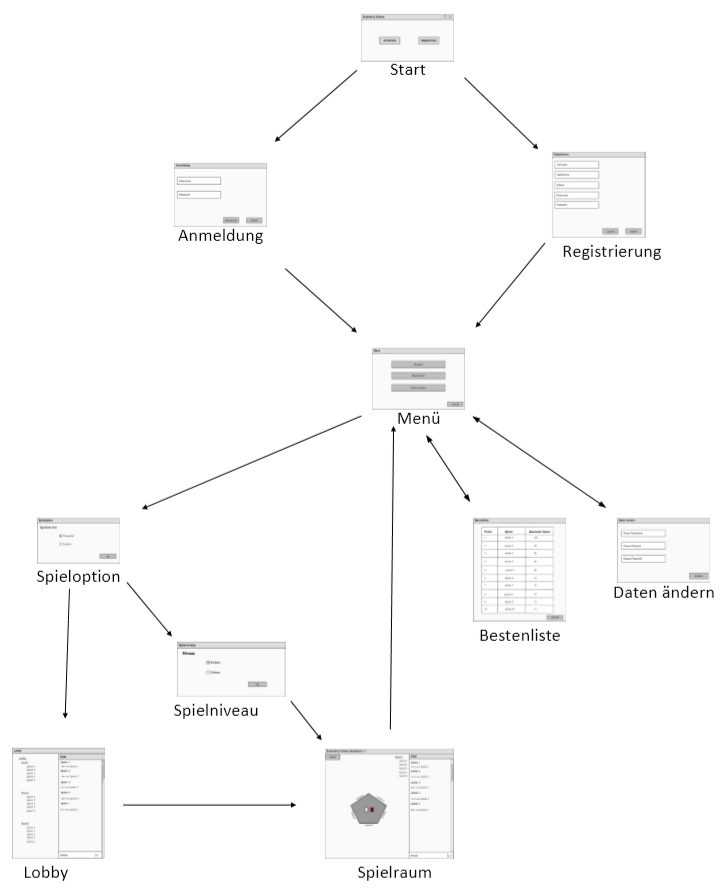
\includegraphics[width=0.9\textwidth]{img/Graph}
	\caption{Darstellung der Zusammenhänge zwischen GUI-Ansichten.}
	\label{gui:zusammenhang}
\end{figure}

\begin{figure}
	\centering
	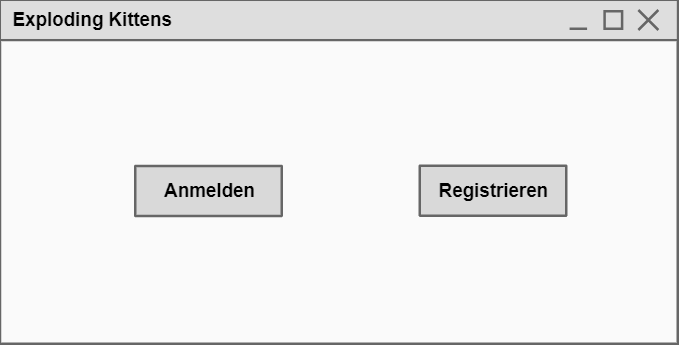
\includegraphics[width=0.5\textwidth]{img/Launch}
	\caption{Skizze für das Startfenster des Programms.}
	\label{gui:start}
\end{figure}

\begin{figure}
	\centering
	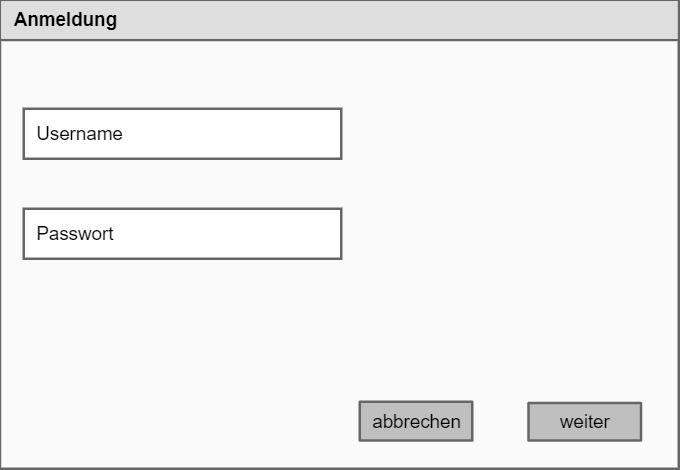
\includegraphics[width=0.5\textwidth]{img/Anmelden}
	\caption{Skizze für das Anmeldefenster.}
	\label{gui:login}
\end{figure}

\begin{figure}
	\centering
	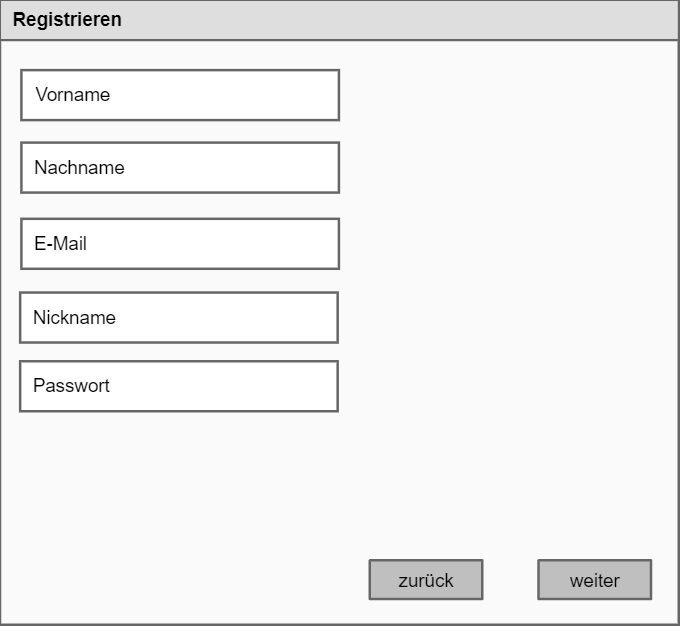
\includegraphics[width=0.5\textwidth]{img/Registrieren}
	\caption{Skizze für das Registrierungsfenster.}
	\label{gui:register}
\end{figure}

\begin{figure}
	\centering
	\includegraphics[width=0.5\textwidth]{img/Menü}
	\caption{Skizze für das Auswahlmenü.}
	\label{gui:menü}
\end{figure}

\begin{figure}
	\centering
	\includegraphics[width=0.5\textwidth]{img/Daten ändern}
	\caption{Skizze für das Fenster zum ändern der Benutzerdaten.}
	\label{gui:daten}
\end{figure}

\begin{figure}
	\centering
	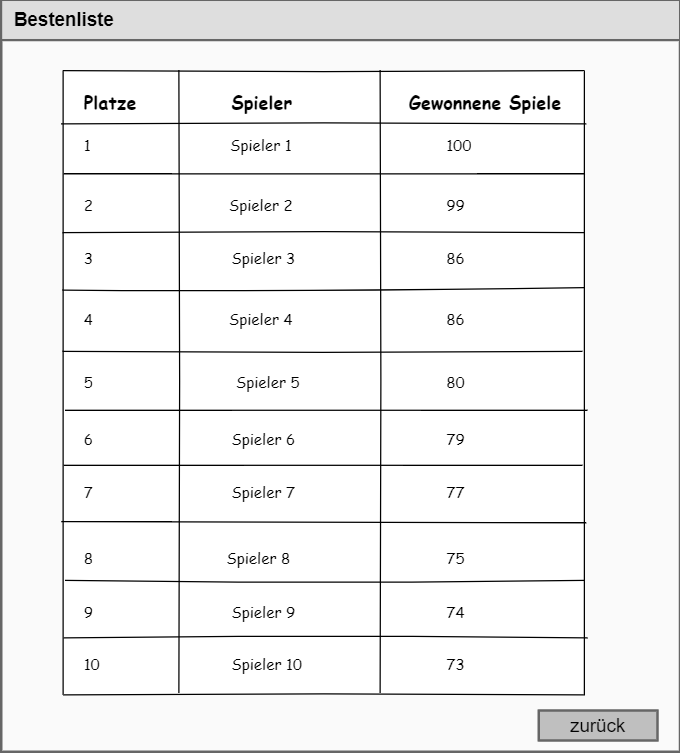
\includegraphics[width=0.5\textwidth]{img/Bestenliste}
	\caption{Skizze für die Bestenliste.}
	\label{gui:bestenliste}
\end{figure}

\begin{figure}
	\centering
	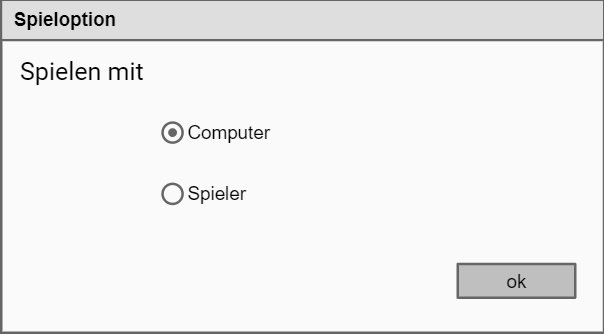
\includegraphics[width=0.5\textwidth]{img/Spieloption}
	\caption{Skizze für das Auswahlfenster zwischen Bots und echten Spielern.}
	\label{gui:option}
\end{figure}

\begin{figure}
	\centering
	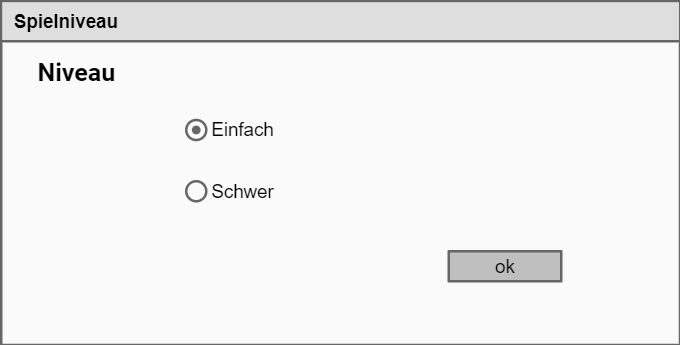
\includegraphics[width=0.5\textwidth]{img/Niveau}
	\caption{Skizze für den Auswahlbildschirm der Bot Schwierigkeit.}
	\label{gui:niveau}
\end{figure}

\begin{figure}
	\centering
	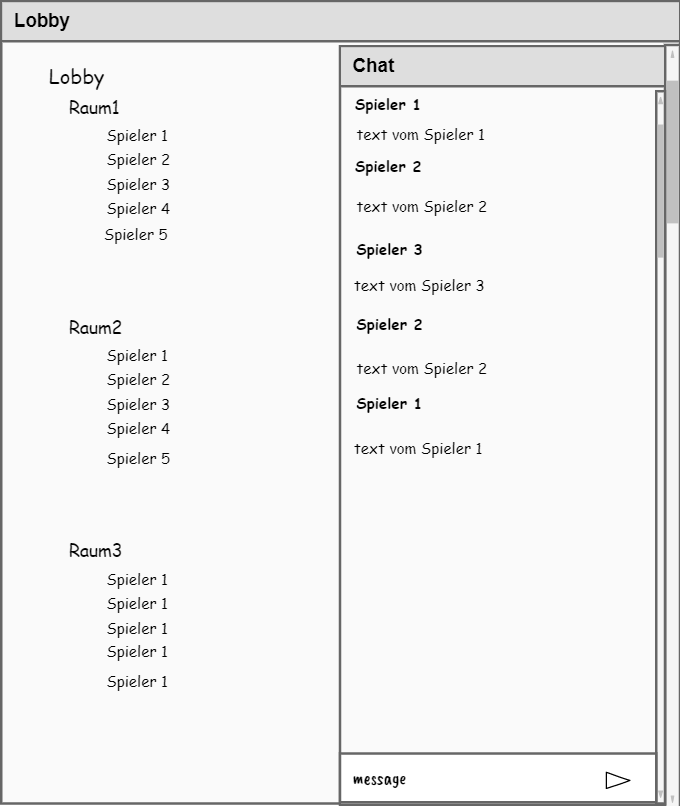
\includegraphics[width=0.5\textwidth]{img/Lobby}
	\caption{Skizze für die Lobby.}
	\label{gui:lobby}
\end{figure}

\begin{figure}
	\centering
	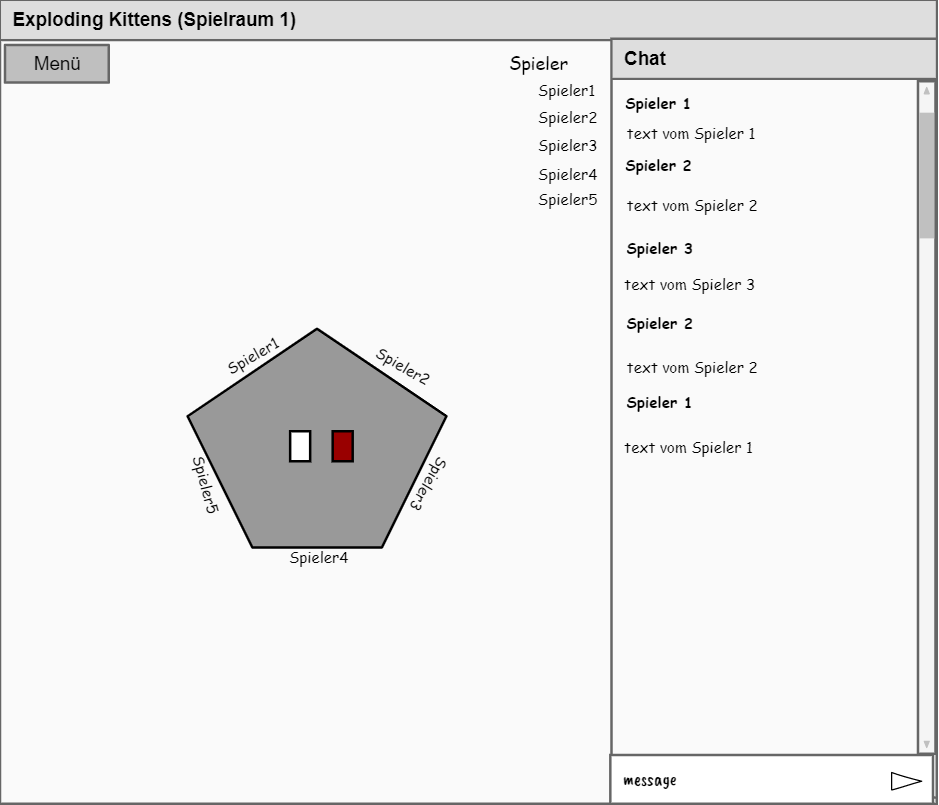
\includegraphics[width=0.5\textwidth]{img/Spielraum}
	\caption{Skizze für den Spielraum.}
	\label{gui:raum}
\end{figure}
	
	\chapter{Systemtestfälle}

Hier sollen verschiedene Szenarien beschrieben werden, mithilfe deren Sie später Systemtests ausführen und die erwarteten Ergebnisse darstellen.

\newcounter{tf}\setcounter{tf}{10}

\begin{description}[leftmargin=5em, style=sameline]

\begin{lhp}{tf}{TF}{tests:anmelden}
	\item [Name:] Spieler anmelden.
	\item [Motivation:] Testet, ob die Anmeldung im System korrekt funktioniert.
	\item [Sczenarien:] \hfill
		\begin{enumerate}
			\item \textit{Zugriffsdaten sind vorhanden und richtig} \\ $\implies$ Spieler wird in die Lobby bewegt.
			\item \textit{Benutzername ist registriert, Passwort ist falsch} \\ $\implies$ Fehlermeldung wird angezeigt.
			\item \textit{Benutzername ist nicht registriert} \\ $\implies$ Fehlermeldung wird angezeigt.
		\end{enumerate}
	\item [Relevante Systemfunktionen:] \ref{funk:zugriff}
	\item [Relevante Use Cases:] \ref{uc:anmeld}
\end{lhp}

\end{description}

\begin{description}[leftmargin=5em, style=sameline]

\begin{lhp}{tf}{TF}{tests:registrieren}
	\item [Name:] Spieler registrieren.
	\item [Motivation:] Testet, ob die Registrierung in dem System korrekt funktioniert.
	\item [Sczenarien:] \hfill
		\begin{enumerate}
			\item \textit{Benutzername sind vorhanden und richtig} \\ $\implies$ Ein Account mit den eingetragenen Daten wird erzeugt und der Spieler wird in die Lobby bewegt.
			\item \textit{Benutzername ist schon genutzt} \\ $\implies$ Fehlermeldung wird angezeigt.
			\item \textit{Email ist schon genutzt} \\ $\implies$ Fehlermeldung wird angezeigt.
		\end{enumerate}
	\item [Relevante Systemfunktionen:] \ref{funk:zugriff}
	\item [Relevante Use Cases:] \ref{uc:anmeld}
\end{lhp}

\end{description}

\begin{description}[leftmargin=5em, style=sameline]

\begin{lhp}{tf}{TF}{tests:account bearbeiten}
	\item [Name:] Account bearbeiten.
	\item [Motivation:] Testet, ob das Bearbeiten des Accounts in dem System korrekt funktioniert.
	\item [Sczenarien:] \hfill
		\begin{enumerate}
			\item \textit{Neuer Benutzername nicht vorhanden} \\ $\implies$ Benutzername wird erfolgreich geändert.
			\item \textit{Neuer Benutzername  bereits vorhanden} \\ $\implies$ Fehlermeldung wird angezeigt.
			\item \textit{Neues Passwort bearbeiten, altes richtig} \\ $\implies$ Passwort wird erfolgreich geändert.
			\item \textit{Neues Passwort bearbeiten, altes falsch} \\ $\implies$ Fehlermeldung wird angezeigt.
			\item \textit{Profil Bild bearbeiten} \\ $\implies$ Profil Bild wird erfolgreich geändert.
			\item \textit{Profil Bild bearbeiten funktioniert nicht} \\ $\implies$ Fehlermeldung wird angezeigt.
		\end{enumerate}
	\item [Relevante Systemfunktionen:] \ref{funk:zugriff}
	\item [Relevante Use Cases:] \ref{uc:anmeld}
\end{lhp}

\end{description}

\begin{description}[leftmargin=5em, style=sameline]

\begin{lhp}{tf}{TF}{tests:account löschen}
	\item [Name:] Account löschen.
	\item [Motivation:] Testet, ob das Löschen des Accounts in dem System korrekt funktioniert.
	\item [Sczenarien:] \hfill
		\begin{enumerate}
			\item \textit{Passwort richtig} \\ $\implies$ Spieler wird in den Anmeldebildschirm bewegt, Account wird gelöscht.
			\item \textit{Passwort falsch} \\ $\implies$ Fehlermeldung wird angezeigt.
	
		\end{enumerate}
	\item [Relevante Systemfunktionen:] \ref{funk:zugriff}
	\item [Relevante Use Cases:] \ref{uc:anmeld}
\end{lhp}

\end{description}

\begin{description}[leftmargin=5em, style=sameline]

\begin{lhp}{tf}{TF}{tests:Spielraum}
	\item [Name:] Spielraum erstellen,bearbeiten oder löschen.
	\item [Motivation:] Testet, ob das Erstellen,das Bearbeiten oder das Löschen eines Spielraums im System korrekt funktioniert.
	\item [Sczenarien:] \hfill
		\begin{enumerate}
			\item \textit{Spielraum erstellt} \\ $\implies$ Spieler wird im erstellte Spielraum bewegt.
			\item \textit{Spielraum erstellt funktioniert nicht} \\ $\implies$ Fehlermeldung wird angezeigt und kein Spielraum wird erstellt.
			\item \textit{Spielraum bearbeiten} \\ $\implies$ Spielraum Eigenschaften werden geändert.
			\item \textit{Spielraum bearbeiten funktioniert nicht} \\ $\implies$ Fehlermeldung wird angezeigt.
			\item \textit{Spielraum löschen} \\ $\implies$ Spieler soll das Löschen bestätigen.
							         \\ $\implies$ Spieler wird im Spiel Menü bewegt.
\\ $\implies$ Spielraum wird gelöscht.
			\item \textit{Spielraum löschen funktioniert nicht} \\ $\implies$ Fehlermeldung wird angezeigt.
\\ $\implies$ Spielraum wird nicht gelöst.
		\end{enumerate}
	\item [Relevante Systemfunktionen:] \ref{funk:zugriff}
	\item [Relevante Use Cases:] \ref{uc:anmeld}
\end{lhp}

\end{description}

\begin{description}[leftmargin=5em, style=sameline]

\begin{lhp}{tf}{TF}{tests:Bots }
	\item [Name:] Bots.
	\item [Motivation:] Testet, ob das Hinzufügen bzw. das Entfernen der Bots korrekt funktioniert.
	\item [Sczenarien:] \hfill
		\begin{enumerate}
			\item \textit{Bots hinzufügen, Platz vorhanden} \\ $\implies$ Bots werden im Spielraum bewegt.
			\item \textit{Bots hinzufügen, kein Platz vorhanden} \\ $\implies$ Fehlermeldung wird angezeigt.
			\item \textit{Bots entfernen, Bot im Raum} \\ $\implies$ Bots werden entfernt.
			\item \textit{Bots entfernen, kein Bot im Raum} \\ $\implies$ Fehlermeldung wird angezeigt.
		\end{enumerate}
	\item [Relevante Systemfunktionen:] \ref{funk:zugriff}
	\item [Relevante Use Cases:] \ref{uc:anmeld}
\end{lhp}

\end{description}

\begin{description}[leftmargin=5em, style=sameline]

\begin{lhp}{tf}{TF}{tests:Spiel}
	\item [Name:] Spiel.
	\item [Motivation:] Testet, ob das Starten bzw. das Ende des Spiels korrekt funktioniert.
	\item [Sczenarien:] \hfill
		\begin{enumerate}
			\item \textit{Spiel starten, genug Spieler} \\ $\implies$ Spiel starten.
														\\ $\implies$ Spieler werden im Spielraum bewegt.
			\item \textit{Spiel starten, nicht genug Spieler} \\ $\implies$ Fehlermeldung wird angezeigt.
			\item \textit{Spiel beenden funktioniert} \\ $\implies$ Spiel wird  beendet.
													  \\ $\implies$ Spieler werden  in Lobby bewegt.
			\item \textit{Spiel beenden funktioniert nicht} \\ $\implies$ Fehlermeldung wird angezeigt.
		\end{enumerate}
	\item [Relevante Systemfunktionen:] \ref{funk:zugriff}
	\item [Relevante Use Cases:] \ref{uc:anmeld}
\end{lhp}

\end{description}


\begin{description}[leftmargin=5em, style=sameline]

\begin{lhp}{tf}{TF}{tests:Bestenliste}
	\item [Name:] Bestenliste.
	\item [Motivation:] Testet, ob das Anzeigen der Bestenliste  korrekt funktioniert.
	\item [Sczenarien:] \hfill
		\begin{enumerate}
			\item \textit{Bestenliste anzeigen, mindestens ein Spiel abgeschlossen} \\ $\implies$ Bestenliste anzeigen.
			\item \textit{Bestenliste anzeigen, bisher niemand gespielt} \\ $\implies$ Fehlermeldung wird angezeigt.
		\end{enumerate}
	\item [Relevante Systemfunktionen:] \ref{funk:zugriff}
	\item [Relevante Use Cases:] \ref{uc:anmeld}
\end{lhp}

\end{description}


\begin{description}[leftmargin=5em, style=sameline]

\begin{lhp}{tf}{TF}{tests: Chatroom}
	\item [Name:] Chatroom.
	\item [Motivation:] Testet, ob das Empfangen bzw. das Senden von Nachrichten korrekt funktioniert.
	\item [Sczenarien:] \hfill
		\begin{enumerate}
			\item \textit{Nachricht schicken, mit Inhalt} \\ $\implies$ Nachricht wird verschickt und erscheint im Chatfenster aller Spieler.
			\item \textit{Nachricht schicken, kein Inhalt} \\ $\implies$ Fehlermeldung wird angezeigt.
										\\ $\implies$Keine Nachricht wird verschickt.
		\end{enumerate}
	\item [Relevante Systemfunktionen:] \ref{funk:zugriff}
	\item [Relevante Use Cases:] \ref{uc:anmeld}
\end{lhp}

\end{description}


\begin{description}[leftmargin=5em, style=sameline]

\begin{lhp}{tf}{TF}{tests:Spieler einladen}
	\item [Name:] :Spieler einladen.
	\item [Motivation:] Testet, ob man Spieler einladen kann.
	\item [Sczenarien:] \hfill
		\begin{enumerate}
			\item \textit{Spieler wird zum Spiel eingeladen, Spieler existiert} \\ $\implies$ Spiel starten mit Freunden.
			\item \textit{Spieler wird zum Spiel eingeladen, Spieler existiert nicht} \\ $\implies$ Fehlermeldung wird angezeigt.

		\end{enumerate}
	\item [Relevante Systemfunktionen:] \ref{funk:zugriff}
	\item [Relevante Use Cases:] \ref{uc:anmeld}
\end{lhp}

\end{description}

\begin{description}[leftmargin=5em, style=sameline]

\begin{lhp}{tf}{TF}{tests: Spieler Punkte }
	\item [Name:] Spieler Punkte.
	\item [Motivation:] Testet, ob die Spielers Punkte übertragen werden.
	\item [Sczenarien:] \hfill
		\begin{enumerate}
			\item \textit{Das Spiel ist fertig. Kein Spielabbruch.} \\ $\implies$ Verdiente Punkte werden zu den vorherigen Punkte addiert.
			\item \textit{Das Spiel ist fertig. Spielabbruch.} \\ $\implies$ Keine Punkte werden zu den vorherigen Punkte addiert.
		\end{enumerate}
	\item [Relevante Systemfunktionen:] \ref{funk:zugriff}
	\item [Relevante Use Cases:] \ref{uc:anmeld}
\end{lhp}

\end{description}































	\chapter{Warteraum}

Hier werden Anforderungen spezifiziert die den sogenannten ``Warteraum'' darstellen. Hier gehören alle Anforderungen, die ``Wünschkriterien'' sind, das heißt, sie sind zwar erwünscht, aber werden nur dann in aktuelle Anforderungen übernommen, wenn dafür genügendes Zeitbudget vorhanden ist und werden am wahrscheinlichsten in der Zukunft (und nicht jetzt) implementiert (oder in den kommenden Sprints beim SCRUM-Prozessmodell).

\newcounter{wr}\setcounter{wr}{10}

\begin{description}[leftmargin=5em, style=sameline]	
	\begin{lhp}{wr}{WR}{wr:musik}
		\item [Name:] Hintergrundmusik
		\item [Beschreibung:] Für die Spieler soll eine Auswahl zur Verfügung stehen, mit der die Hintergrundmusik beim Spielen ausgewählt werden kann.
		\item [Motivation:] Höhere Zufriedenheit der Benutzer.
		\item [Erfüllungskriterium:] Spieler können zu jedem Zeitpunkt (außer im Vorraum) die Musik ausschalten oder ein anderes Lied auswählen.
	\end{lhp}
\end{description}
	
\end{document}
